 \documentclass[10pt,article]{IEEEtran}
\usepackage{cite}
\usepackage[cmex10]{amsmath}
\usepackage{array}
\usepackage{url}
\usepackage{graphicx}
\usepackage{graphics}
\usepackage{lmodern}
\begin{document}
\title{An Overview of Network Troubleshooting With SDN}

%\author{\IEEEauthorblockN{Knop Thibaut}
%\IEEEauthorblockA{Ecole polytechnique de Louvain\\
%Université Catholique de Louvain\\
%Louvain-la-Neuve, Belgique\\
%Email: thibaut.knop@student.uclouvain.be}
%\and
%\IEEEauthorblockN{Rochet Florentin}
%\IEEEauthorblockA{Ecole polytechnique de Louvain\\
%Université Catholique de Louvain\\
%Louvain-la-Neuve, Belgique\\
%Email: florentin.rochet@student.uclouvain.be}}

\maketitle
\begin{abstract}
TODO
\end{abstract}

\begin{IEEEkeywords}
TODO
\end{IEEEkeywords}

\section{Introduction}
%Rappel sur SDN (a NICE way)
%Qu'est ce qui créé les erreurs dans les SDN networks (a NICE way, page 1 et 2)

Since years, the main problem in network maintenance is network debugging. Bugs are really difficult to spot with tools like ping, traceroute and SNMP agents, which are the most used to diagnose issues. \cite{...}\\ %27 dans leveraging ...
Hopefully, this could change thanks to the deployment of Software-Defined Networks. SDN is an architecture developped to fix the mess in the control plane. It acts like a logically-centralized controller which manages switches by installing (or uninstalling) rules in them. The controller also read traffic statistics and respond to events. An handler is attached for each events and respond to its event by applying the routine establised by the network engineer. \\
Thanks to SDN, it should be possible to automate troubleshooting, this will be seen in (TODO: how to reference to a next section ?).

\section{SDN layering, the key used to a better troubleshooting}
 % Expliquer ici la stack SDN (decomposition en layer) et donner l'intuition concernant la plus grande facilité pour remonter à l'origine d'un probleme.
Finding and solving network bugs are not the aim of SDN, but we can use it to re-think the way we troubleshoot networks.\\ The SDN architecture is decomposed into  layers, those layers can be represented in a two dimensionnal array. As you can see on Figure \ref{layers}, we have the two main layers called \textit{State layers} and \textit{Code layers}. The state layers hold a representation of the network's configuration for each parts of the network architecture. The code layers implement logic to maintain the mapping between two state layers. Each states layers should verify the equivalence properties, which means that each of them should correctly mapping every other state layer. The idea is that, for each policy, if the state layers are correctly mapped among each other, then the policy is  set and acts like it should.\\
Thus, thanks to the SDN stack, we are able to first build a tool to check consistency between state layers in order to identify on which part of the network architecture a bug is happening. \\
When the layer is identified, an other tool take over to localize the issue inside the code layer. We will see in (TODO: indicates next section) which kind of tools could be used to handle that.
\begin{itemize}
\item explication graphique
\item plus en détail finding the code layer and finding within the code layer. (summary)
\end{itemize}
\begin{figure}
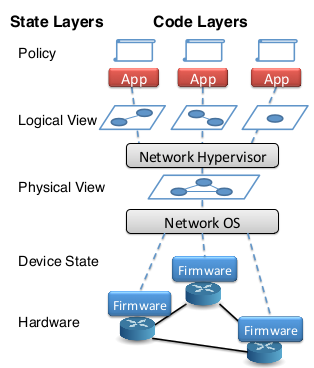
\includegraphics[scale=0.65]{layers.png}
\label{layers}
\caption{SDN architecture}
\end{figure}
\section{Network Troubleshooting - Tools}

\subsection{tool1 - 1 subsection par tool}
\begin{itemize}
\item NDB - présenter un outil pour finding the code layer
\item Veriflow
\item Soft
\item Nice
\item FlowChecker ?
\end{itemize}
Expliquer ici par rapport au layer\\

voir page 2 a Nice way (challenge pour tester l'open flow) et les solutions qui existent)


\section{Conclusion}
TODO
\nocite{*}
\bibliographystyle{IEEEtran}
\bibliography{IEEEabrv,draft}

\end{document}
